\chapter{Discussion}
\label{chap:discussion}

This chapter synthesizes the findings from Chapter~\ref{chap:results} and evaluates them against the
overall research aim and the three research questions in
Section~\ref{sec:rq}. The discussion links detection and tracking performance to the theoretical framework in Chapter~\ref{chap:theory}, justifies model and tracker selection, and compares the observed results with relevant prior work. It further
examines daytime and nighttime behaviour, live deployment performance, and the practical
implications for intersection planning under Norwegian guidelines (N100 and V121).
Finally, the chapter critically addresses methodological and statistical limitations and
outlines the scope of valid conclusions.




\section{Detection Performance of the Fine-Tuned YOLO26 Models}

The training and validation curves for both YOLO26n and YOLO26m (\autoref{sec:yolo_train_val}) were characterized by a rapid performance increase in the first 10–15 epochs, followed by an early plateau around epoch 55 and subsequent early stopping. This pattern is consistent with the design goals of YOLO26’s training innovations described in Section \autoref{sec:yolo26-advancements}. The Progressive Loss Balancing (ProgLoss) mechanism and the MuSGD optimizer are intended to promote more stable and efficient convergence by dynamically adjusting loss component weighting and improving optimisation behaviour \citep{sapkota2026yolo26keyarchitecturalenhancements}. In the context of this study, the early stabilisation suggests that both models relatively quickly learned the dominant visual features present in the custom dataset. The fact that validation-set performance exceeded the final validation metrics indicates some degree of overfitting.

On the independent test set of 193 images containing 761 object instances, both models demonstrated solid overall performance, with YOLO26m outperforming its smaller counterpart (mAP$^{50}$ = 0.808 vs.\ 0.693; mAP$^{50-95}$ = 0.638 vs.\ 0.556). The results confirm that the models are particularly effective at detecting the dominant ``Car'' class and the larger vehicle categories (Light Truck, Heavy Truck and Semi-trailer), which are critical for extracting vehicle composition data required by Norwegian design guidelines (N100 and V121). However, performance was noticeably weaker for classes with fewer instances such as bicycle and person. A particularly large performance gap was observed for the "Bus" class, where YOLO26m achieved substantially higher scores (AP$^{50}$ = 0.828 vs.\ 0.708), driven mainly by improvements in precision.

\subsubsection*{Limitations of the mAP Metric}
While mean Average Precision (mAP) is the standard benchmark for object detection, its mathematical structure introduces certain biases when applied to imbalanced datasets. Because mAP is calculated as an unweighted macro-average, every category, regardless of its frequency in the dataset, contributes equally to the final score (\autoref{eq:mAP_calc}). The 'Bicycle' class was excluded from the adjusted results in \autoref{tab:mAP_no_bicycle} due to its negligible sample size (\(n=2\)) in the test set and a limited representation in the training data. Given this scarcity, the low AP score likely stems from the model's inability to learn robust features for this category, while also reflecting random variance rather than a generalized performance trend. Removing this outlier allows for a more reliable assessment of the model's proficiency in detecting the primary vehicle classes, which were more comprehensively represented.

\begin{table}[H]
\centering
\caption{Comparison of mAP scores with and without the minority \textit{Bicycle} class.}
\label{tab:mAP_no_bicycle}
\begin{tabular}{|l|cc|cc|}
\hline
& \multicolumn{2}{c|}{\textbf{Full Dataset (8 classes)}} & \multicolumn{2}{c|}{\textbf{Adjusted (7 classes)}} \\ \cline{2-5} 
\textbf{Model} & \textbf{$mAP^{50}$} & \textbf{$mAP^{50-95}$} & \textbf{$mAP^{50}$} & \textbf{$mAP^{50-95}$} \\ \hline
YOLO26n & 0.693 & 0.556 & 0.766 & 0.619 \\ \hline
YOLO26m & 0.808 & 0.638 & 0.852 & 0.680 \\ \hline
\end{tabular}
\end{table}

\subsubsection*{Confusion With the Background}
As presented in the confusion matrices in \autoref{sec:test_results}, the background is often mistaken for objects and vise versa. \autoref{fig:FN_crop}--\autoref{fig:FP_occlusion} show some cases of False Negatives and False Positives that negatively affect the results (YOLO26n). 


\begin{figure}[H]
    \centering
    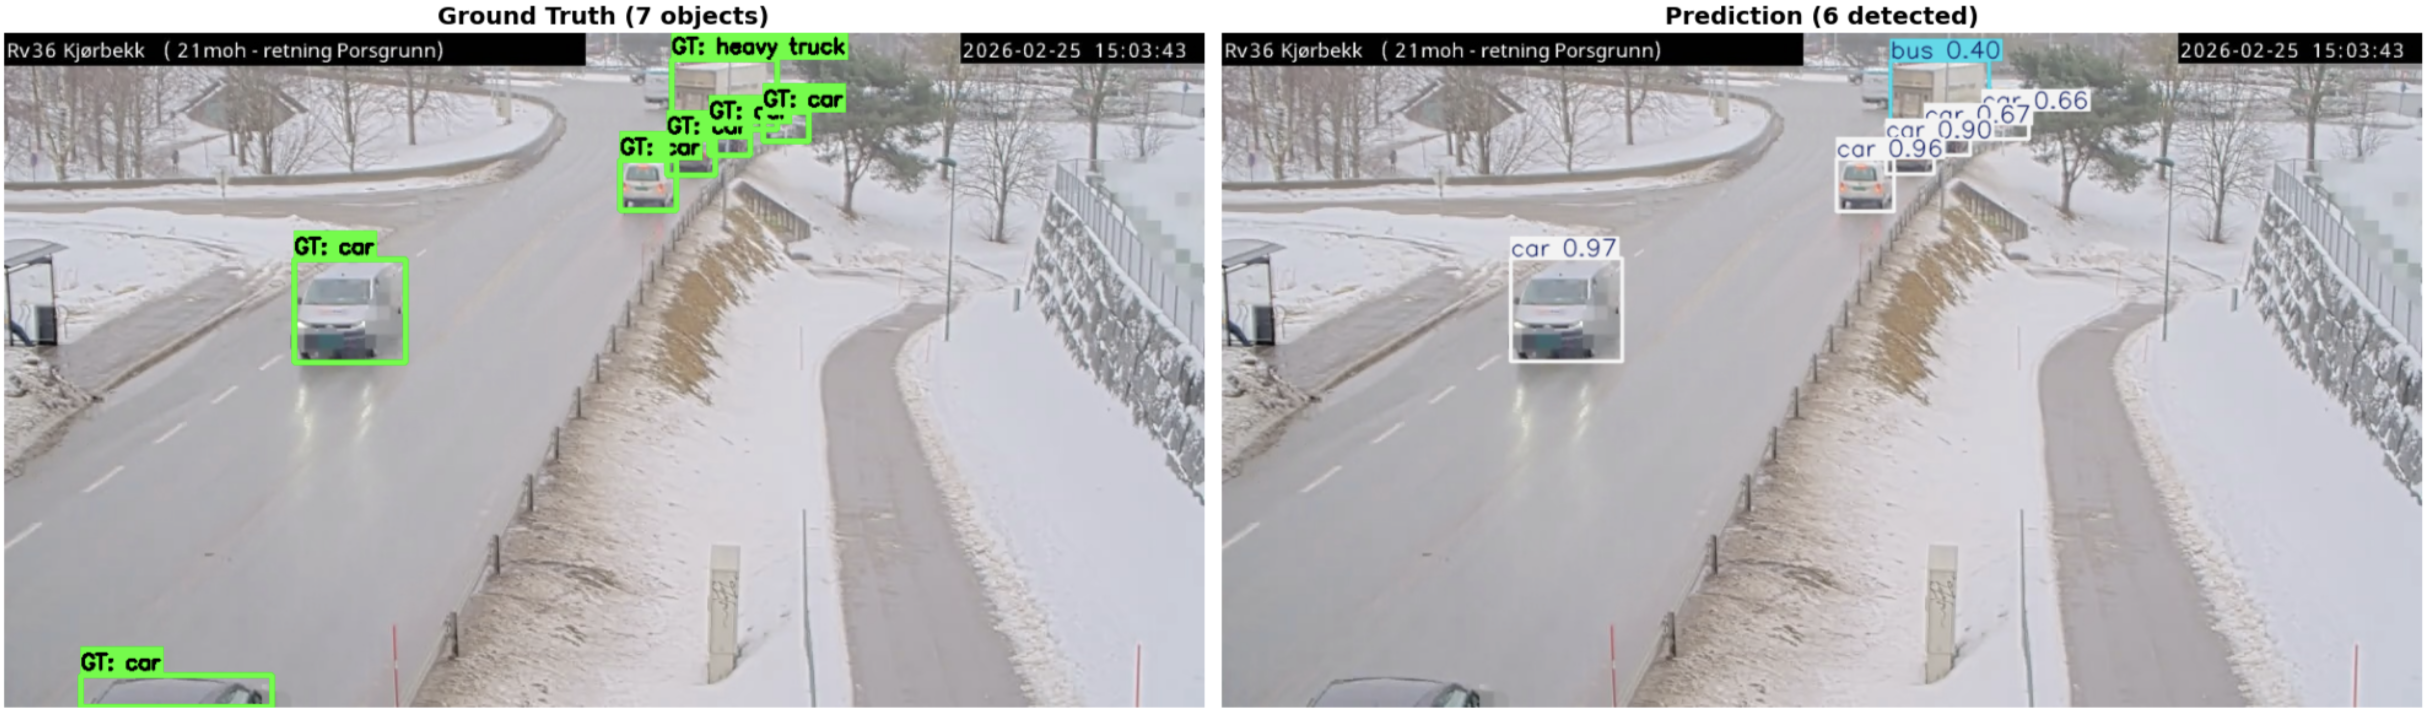
\includegraphics[width=1\linewidth]{project//images/FN_crop.png}
    \caption{\textbf{False Negative:} A car entering the frame from the bottom is annotated, but not predicted.}
    \label{fig:FN_crop}
\end{figure}

\begin{figure}[H]
    \centering
    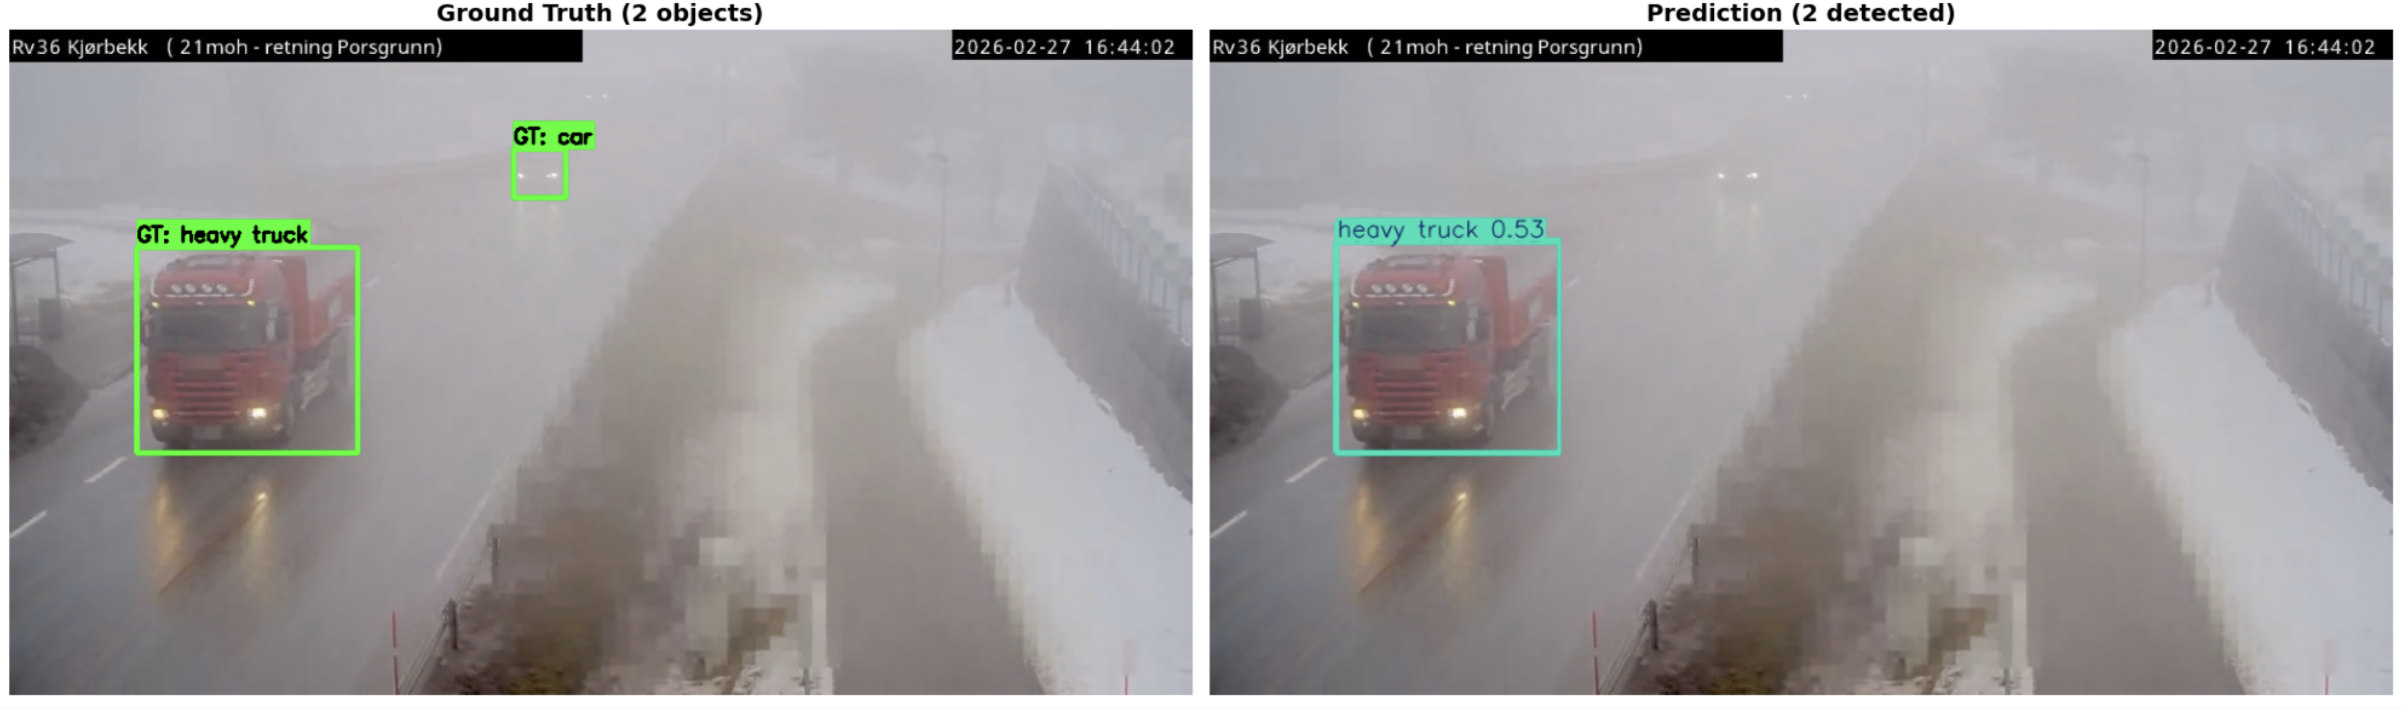
\includegraphics[width=1\linewidth]{project//images/FN_fog.png}
    \caption{\textbf{False Negative:} Missed detection because of foggy weather.}
    \label{fig:FN_fog}
\end{figure}

\begin{figure}[H]
    \centering
    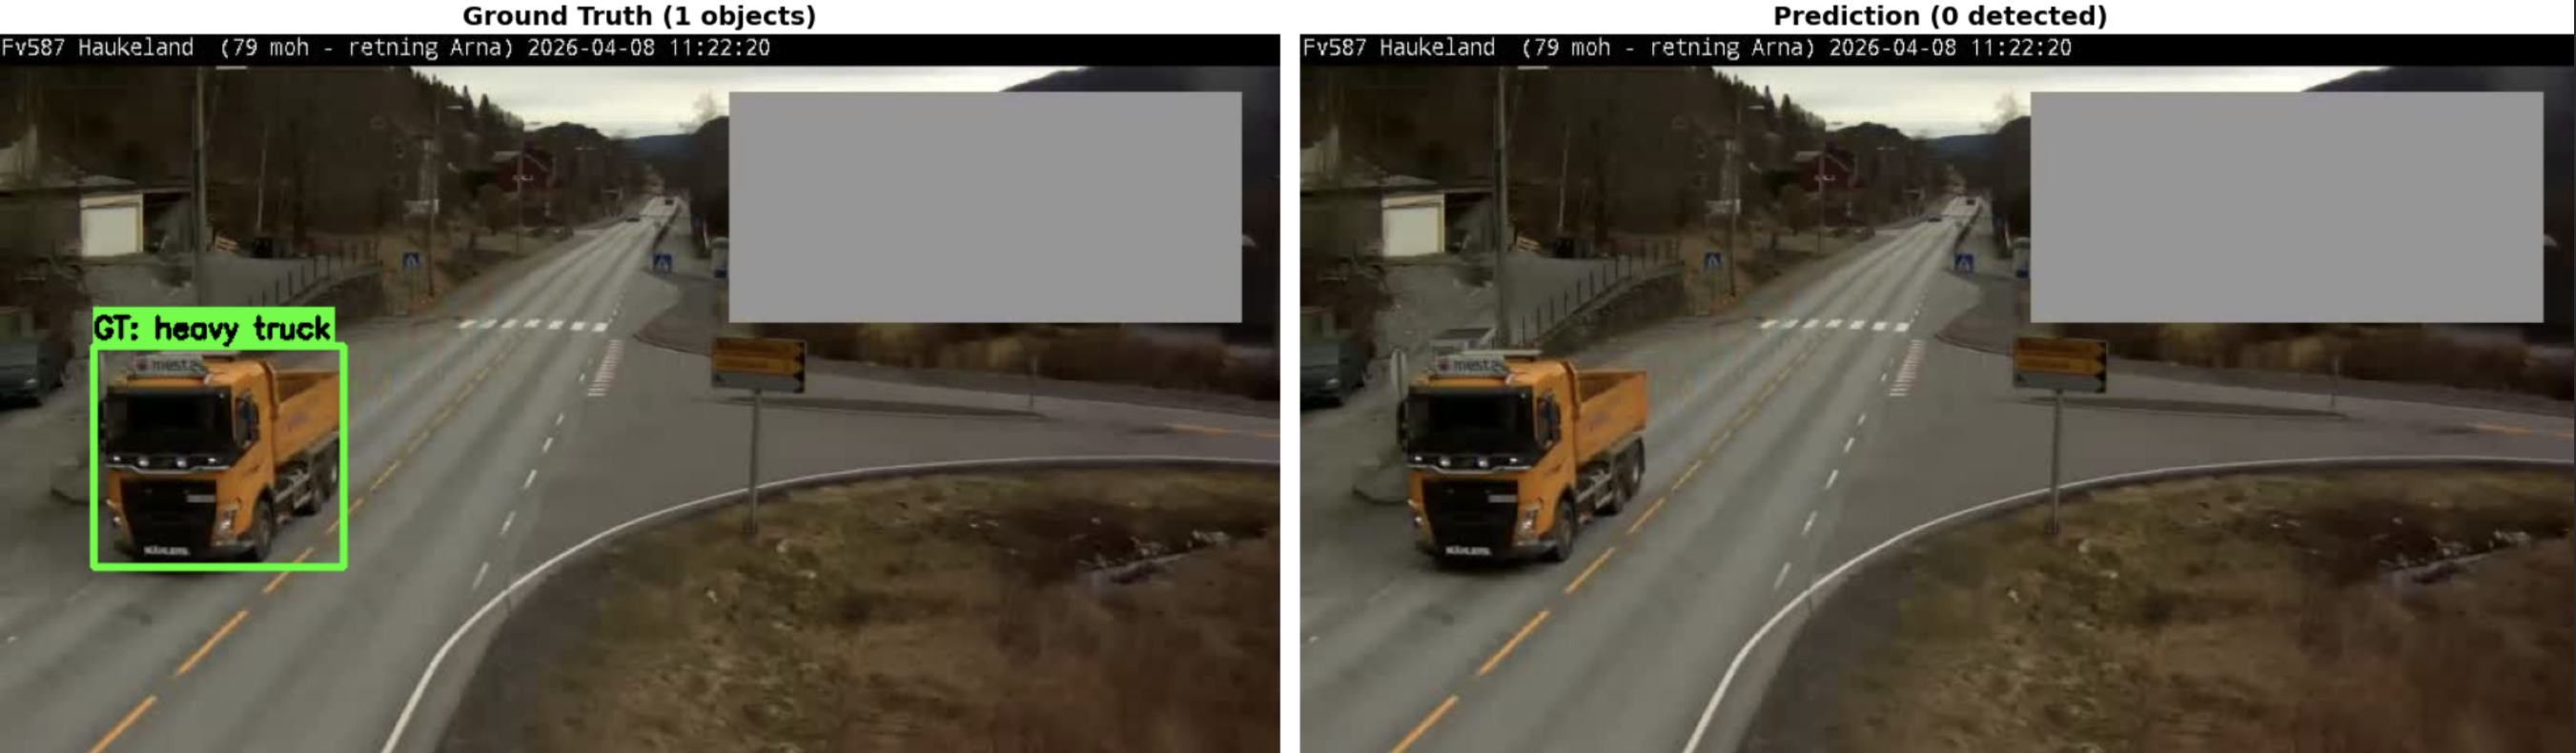
\includegraphics[width=1\linewidth]{project//images/FN_why.png}
    \caption{\textbf{False Negative:} A heavy truck is clearly present, but the model misses it.}
    \label{fig:FN_why}
\end{figure}

\begin{figure}[H]
    \centering
    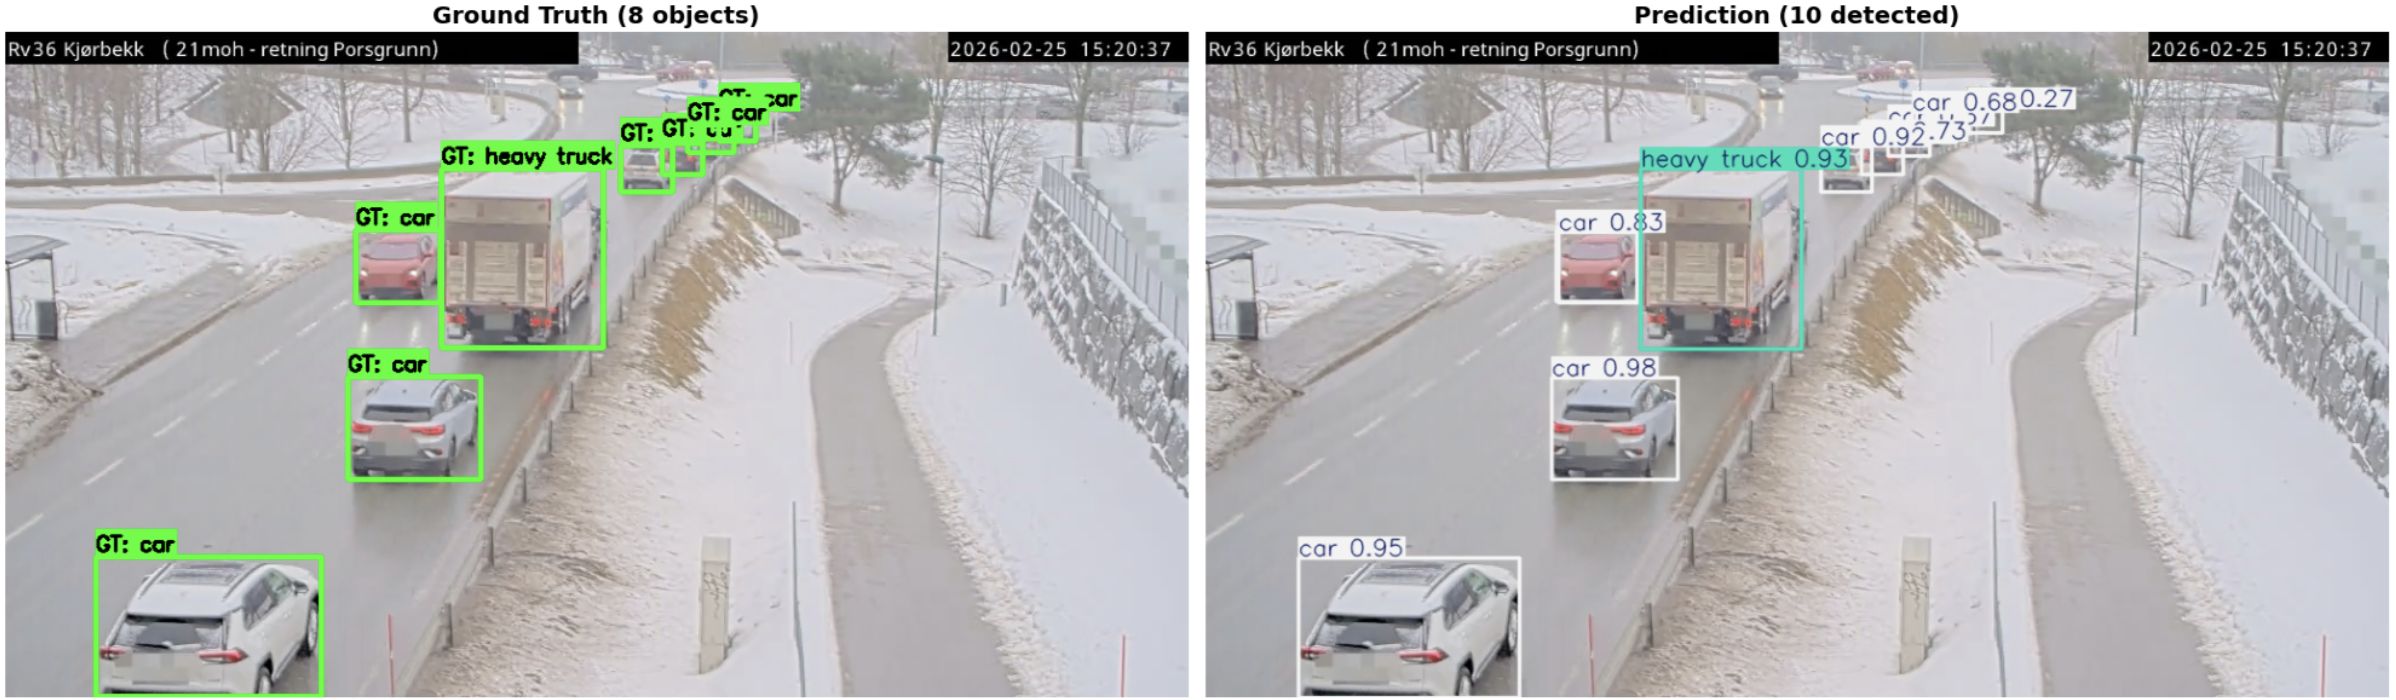
\includegraphics[width=1\linewidth]{project//images/FP_heavy_occlusion.png}
    \caption{\textbf{False Positive:} Heavy occlusion makes the model predict two extra cars on the upper part of the frame.}
    \label{fig:FN_why}
\end{figure}

\begin{figure}[H]
    \centering
    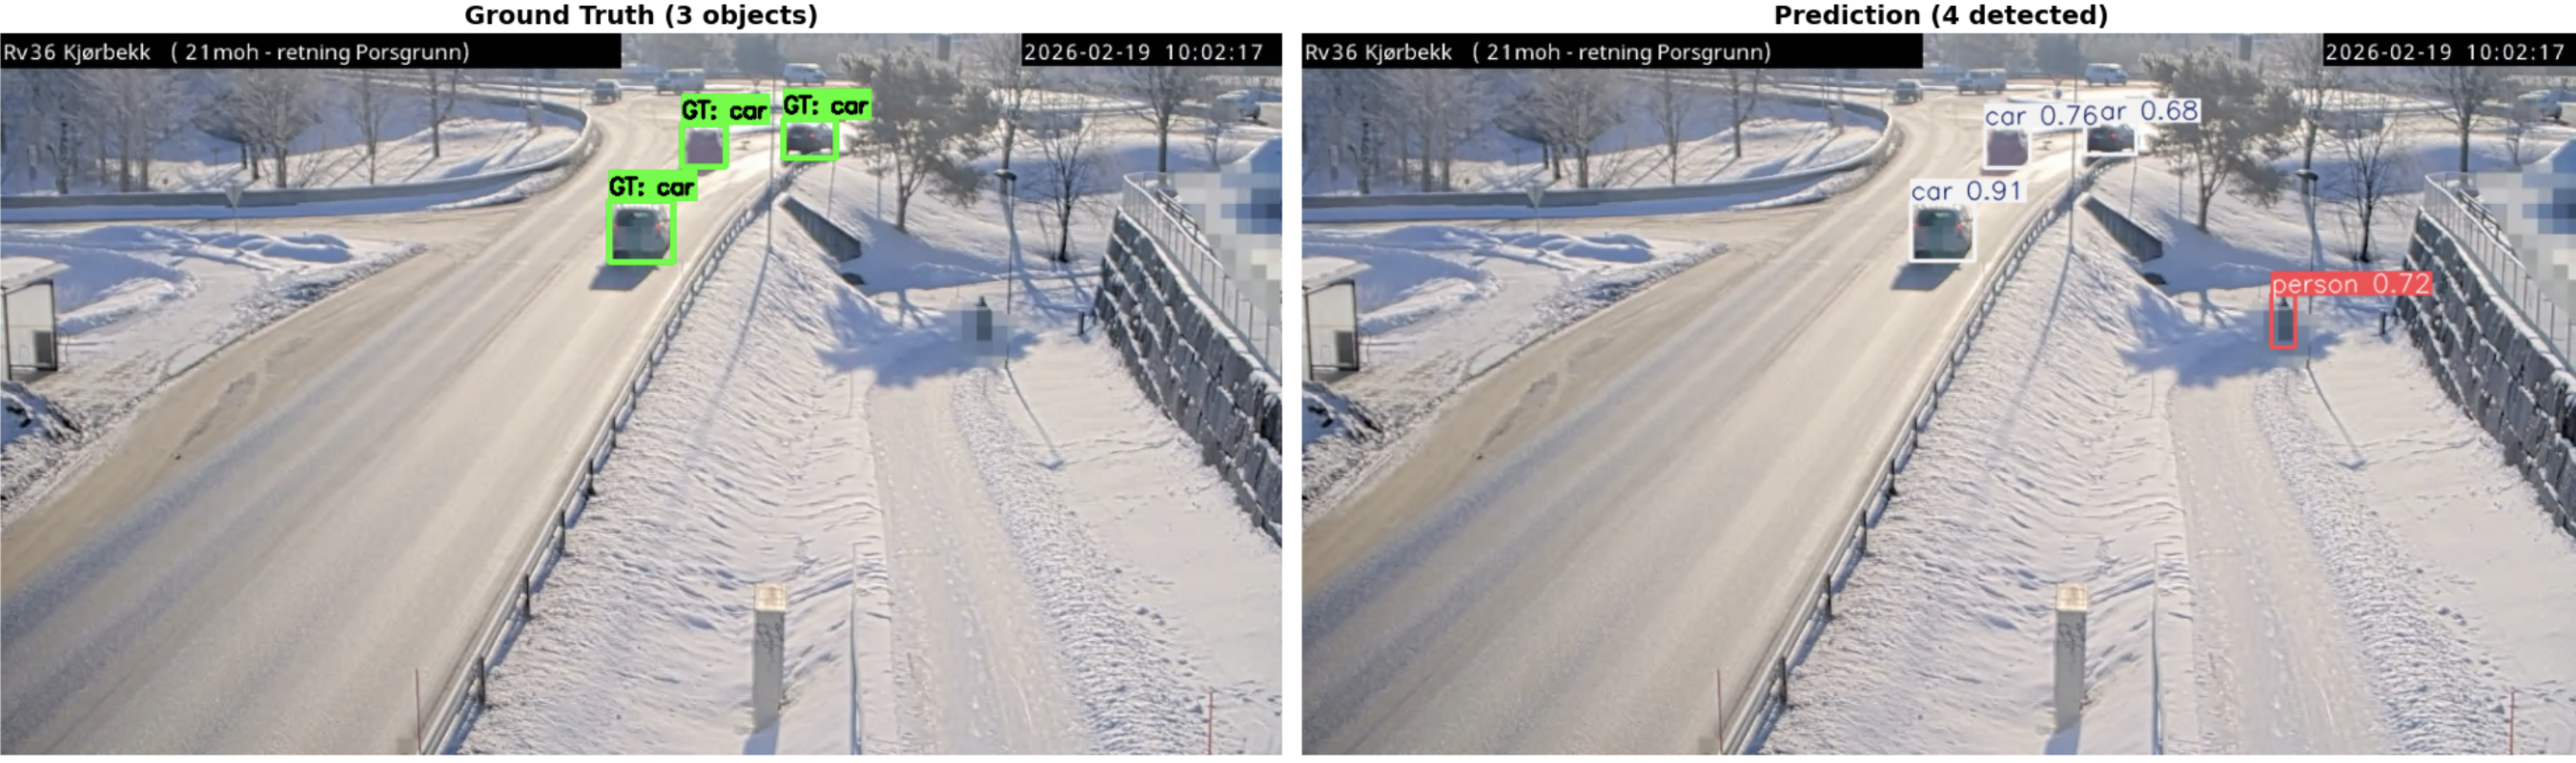
\includegraphics[width=1\linewidth]{project//images/FP_blurry.png}
    \caption{\textbf{False Positive:} A person has gone unnoticed during the annotation, but the model still predicts it.}
    \label{fig:FP_blurry}
\end{figure}

\begin{figure}[H]
    \centering
    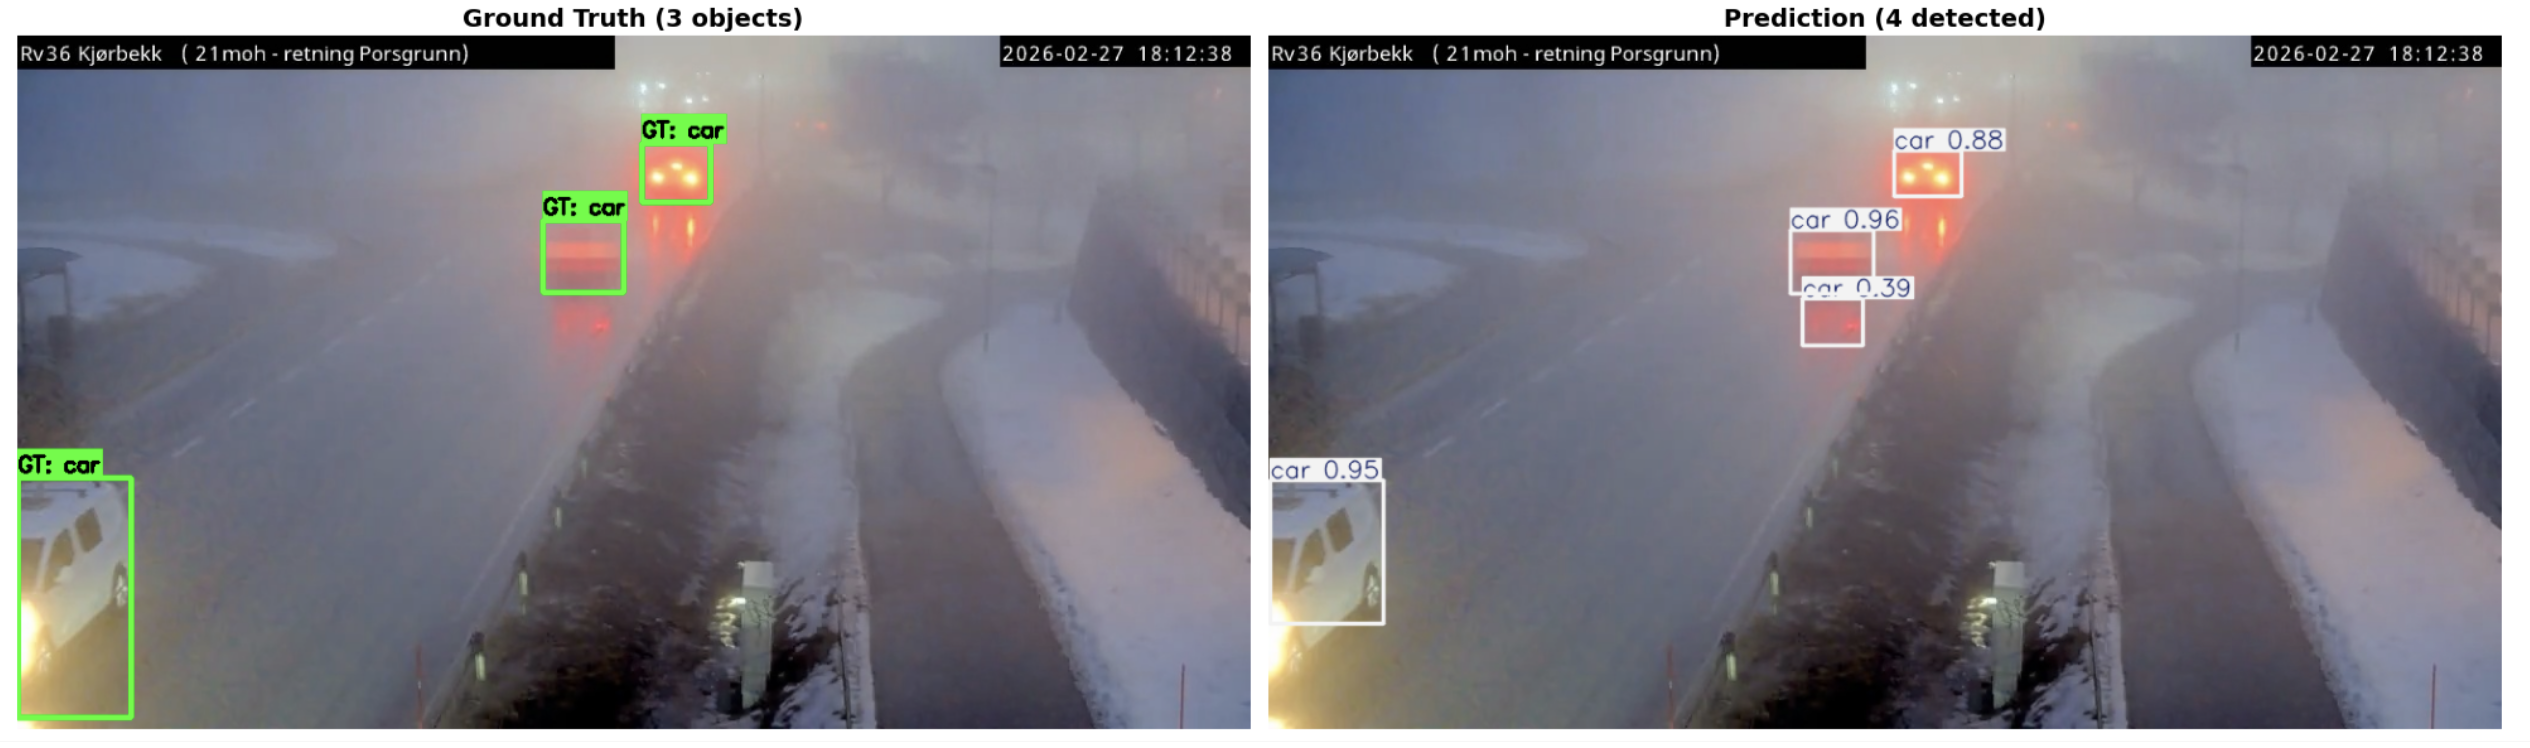
\includegraphics[width=1\linewidth]{project//images/FP_light.png}
    \caption{\textbf{False Positive:} Due to challenging lightning, the model predicts the reflection of a car as an object.}
    \label{fig:FP_light}
\end{figure}

\begin{figure}[H]
    \centering
    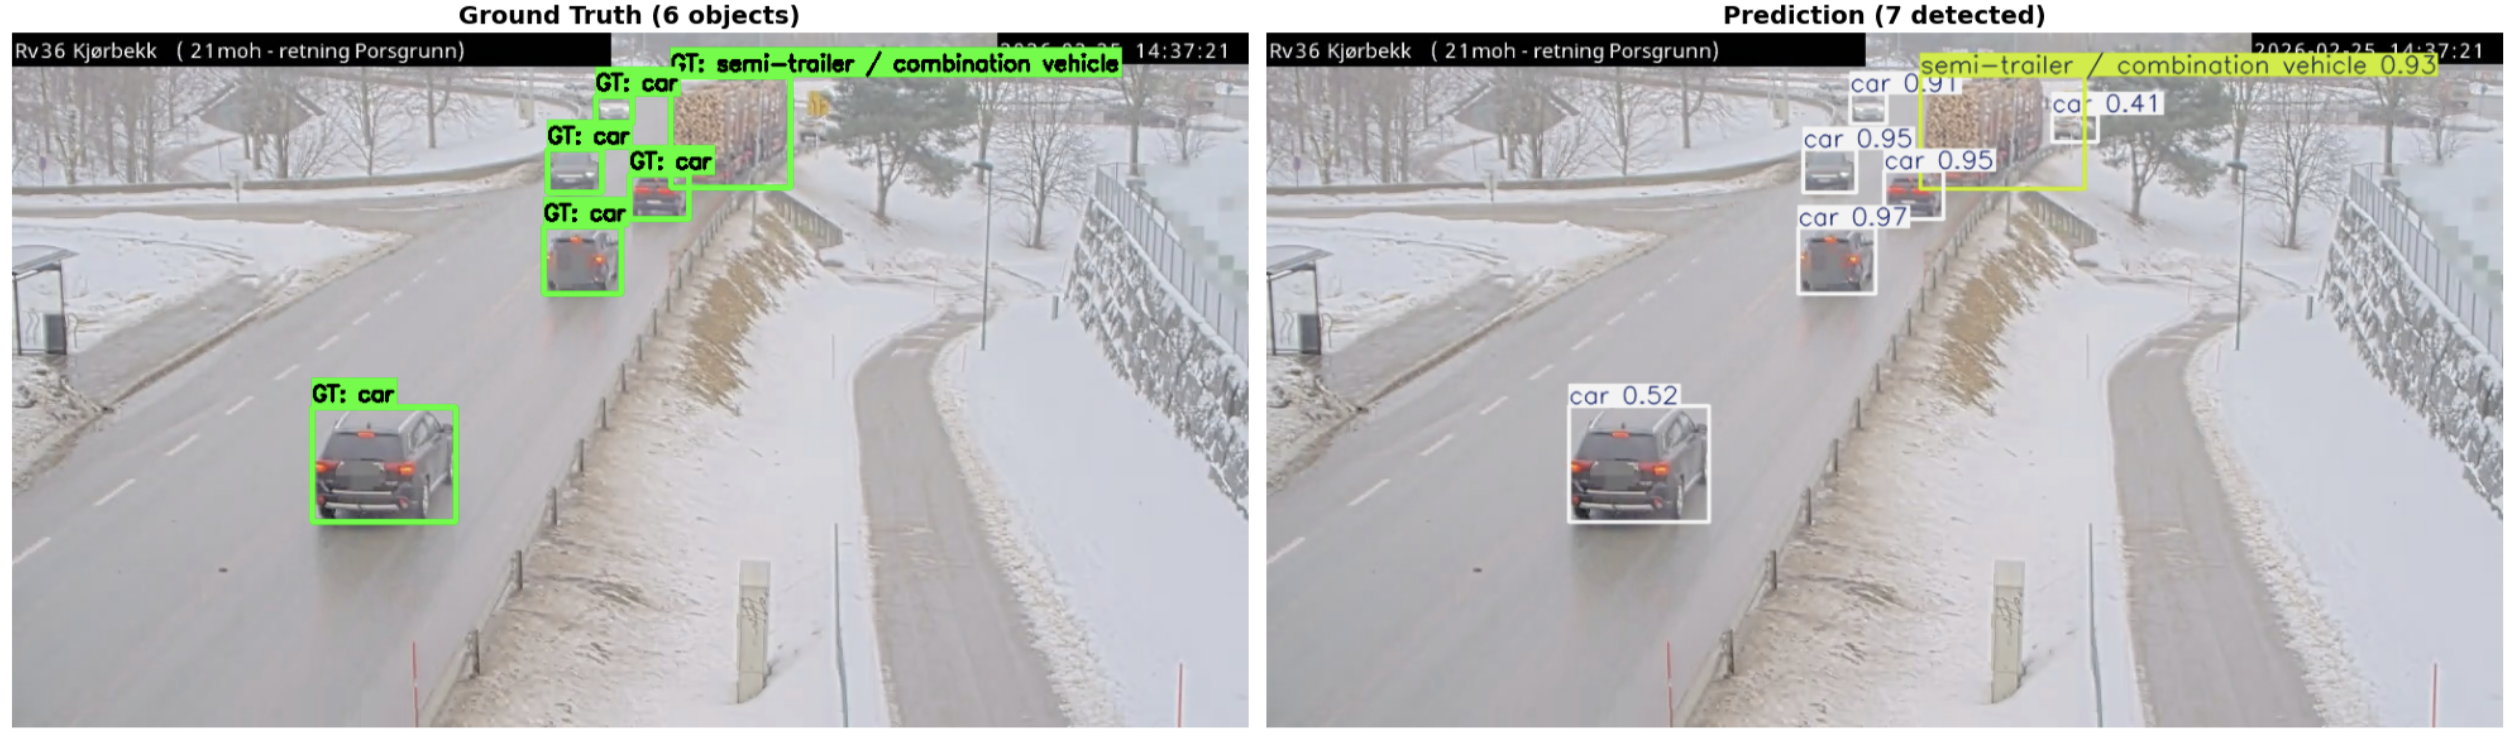
\includegraphics[width=1\linewidth]{project//images/FP_occlusion.png}
    \caption{\textbf{False Positive:} The car on the top right was too far away from the region of interest, so it was not annotated. The model predicts it regardless, even though it is far away and partially occluded.}
    \label{fig:FP_occlusion}
\end{figure}


\subsubsection*{Duplicate Predictions}
Although YOLO26 is designed with a native NMS-free, end-to-end architecture intended to produce unique bounding boxes per object without post-processing, occasional duplicate detections (highly overlapping boxes on the same object) were still observed during inference on the test set. These rare cases typically appear as near-identical predictions with different confidence scores. An example is presented in \autoref{fig:triple_prediction}, where the same pedestrian receives 3 bounding boxes. Only 1 can be counted as a True Positive, and the other 2 are treated as False Positives. This negatively impacts the model's precision.

\begin{figure}[H]
    \centering
    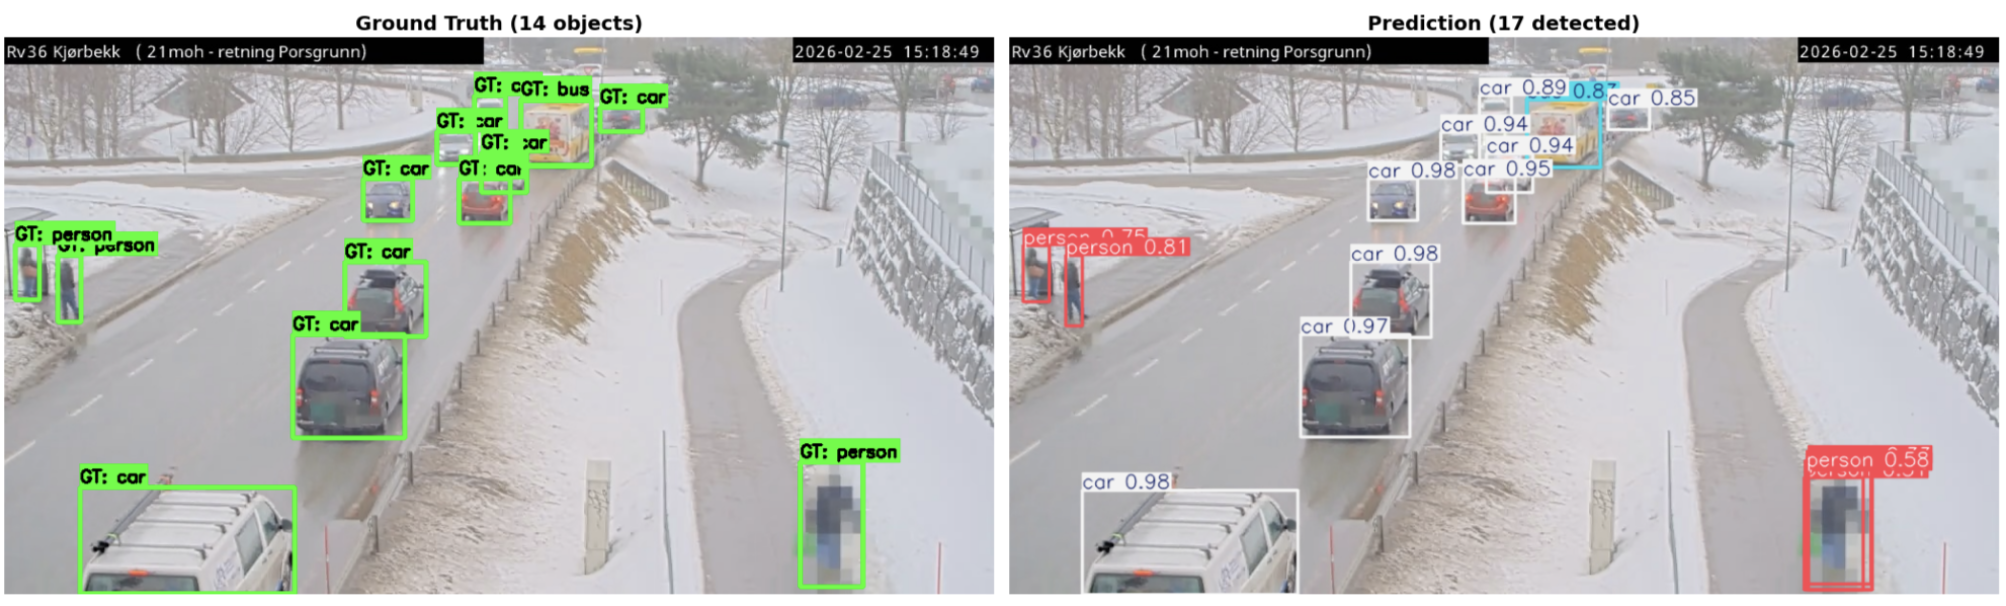
\includegraphics[width=1\linewidth]{project//images/triple_prediction.png}
    \caption{Three predictions on the same pedestrian (bottom right).}
    \label{fig:triple_prediction}
\end{figure}

\subsubsection{Comparison with Prior Work}
Contextualizing these results against published benchmarks reveals the contribution of this study. \cite{YOLO-PEL} introduced YOLOv8-PEL as a lightweight variant of YOLOv8n, achieving 66.9 mAP$^{50}$ with 2.23 M parameters on the COCO-Vehicle dataset. In direct comparison, the YOLO26n model (approximately 2.4 M parameters, 0.693 mAP$^{50}$) and YOLO26m (approximately 20.4 M parameters, 0.808 mAP$^{50}$) demonstrate competitive or superior accuracy despite comparable or slightly higher parameter counts. Notably, our task presented higher inherent difficulty: while the COCO-Vehicle benchmark grouped all heavy vehicles into a single category, we expanded the truck class into three distinct sub-types (Light Truck, Heavy Truck, Semi-trailer), requiring the model to learn finer visual distinctions.

The 0.693 mAP$^{50}$ of YOLO26n already surpasses the 66.9 mAP$^{50}$ baseline from \cite{YOLO-PEL} by approximately 2.4 percentage points on a more challenging multi-class task, while the 0.808 mAP$^{50}$ of YOLO26m represents a substantial further improvement. At the same time, the comparison should be interpreted cautiously: our dataset is substantially smaller (1282 frames) than typical COCO-derived benchmarks (often tens of thousands of images), and the task domain is narrower (intersection-focused vehicle detection rather than general COCO-Vehicle scenes). Accordingly, the main contribution is not only competitive absolute accuracy, but also evidence that domain-specific fine-tuning of modern architectures can deliver operational performance in specialized settings with modest data volumes.

Despite the overall strong performance, qualitative inspection of nighttime footage revealed some missed detections in \autoref{fig:night_pred}. This limitation is consistent with the research gaps identified in Section~\ref{sec:research_gap}, where \cite{DeepLearningTrafficScene2025} emphasise that YOLO-based detectors still require further improvements in small-object detection and robustness under adverse lighting conditions. \cite{YOLO-PEL} similarly stress the importance of practical validation in real-world deployment scenarios, which frequently include challenging illumination.

\begin{figure}[H]
    \centering
    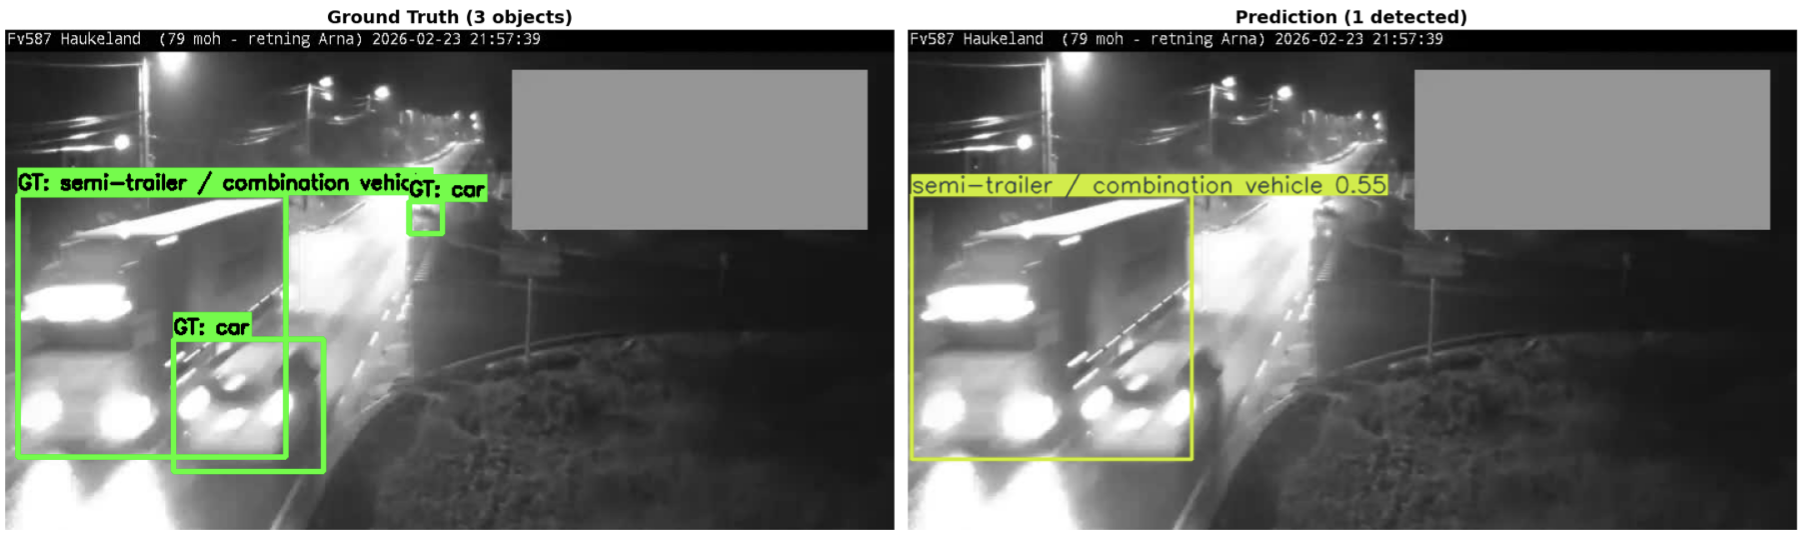
\includegraphics[width=1\linewidth]{project//images/night_pred.png}
    \caption{Missed detections at nighttime.}
    \label{fig:night_pred}
\end{figure}

However, these shortcomings are effectively mitigated in the complete pipeline. By feeding the detections into a multi-object tracker, the model receives multiple temporal opportunities to detect and correctly classify the same vehicle across consecutive frames. This combination significantly increases the chance of successful detection and classification, even when individual frames are difficult. 

\subsection{Model Selection: YOLO26 vs.\ Alternatives}
YOLO26 was selected over contemporary alternatives (YOLOv8, YOLOv11, Faster R-CNN, EfficientDet) for several principled reasons. First, as a one-stage detector, YOLO26 prioritizes real-time inference speed over peak accuracy, which is a critical requirement for continuous intersection monitoring. At the Fv587 Haukeland station, the camera operates at 10 FPS. Downstream processing must complete within 100 ms per frame to remain viable. YOLO26n achieves approximately 26 FPS (ONNX) on standard CPU hardware, providing a 2.6× safety margin, while heavier alternatives like Faster R-CNN typically require GPU acceleration and cannot achieve comparable throughput on CPU.

Second, YOLO26's architectural innovations (Progressive Loss Balancing, MuSGD optimizer, and NMS-free design as discussed in Section~\ref{sec:yolo26-advancements}) directly address challenges inherent to traffic monitoring. The ProgLoss mechanism dynamically balances detection, classification, and localization losses across training, enabling the model to learn fine-grained vehicle class distinctions (e.g., light vs.\ heavy truck) despite severe class imbalance in the dataset. The MuSGD optimizer provides more stable convergence than traditional SGD or Adam variants, as evidenced by the smooth training curves observed in Section~\ref{sec:yolo_train_val}. The NMS-free design eliminates the need to manually tune confidence and IoU thresholds, which is a significant practical advantage over YOLOv8 and earlier variants.

Third, extensive deployment experience with YOLO models in traffic applications \citep{YOLO-PEL, DeepLearningTrafficScene2025} validates the architectural family's suitability for this domain. The custom vehicle-class support demonstrated in this study (light truck, heavy truck, semi-trailer) aligns with YOLO's demonstrated flexibility across diverse object detection tasks.


\section{Tracking Performance}

The fine-tuned YOLO26 models were integrated into the complete tracking pipeline described in Section~\ref{subsec:method_tracking_od}. This section evaluates how detection quality, tracker selection, and environmental conditions (daytime vs.\ nighttime) collectively affect vehicle trajectory reconstruction and origin--destination counting. Four tracking experiments were conducted: a 15-minute daytime segment for tracker configuration selection, a 1-hour daytime segment for main performance evaluation, a 1-hour nighttime segment for low-light evaluation, and a 10-minute twilight segment for adaptive dual-tracker validation. All videos were recorded at the Fv587 Haukeland intersection.

\subsection{Detection Quality as the Limiting Factor in Tracking}

The tracking results demonstrate that overall system performance is fundamentally constrained by detection quality rather than tracker choice. Across the 15-minute daytime configuration selection (Table~\ref{tab:od_daytime_all}), YOLO26m consistently outperforms YOLO26n regardless of tracker algorithm, with Cell MAE improvements of 0.12–0.26 vehicles depending on the tracker variant. This suggests that the nano model's smaller capacity becomes a performance bottleneck when tracking challenging scenarios with occlusions and rapid dynamics. Conversely, tracker selection among YOLO26m configurations shows minimal impact: Day BoT-SORT achieves a Cell MAE of 0.048 compared to 0.143 for both ByteTrack and default BoT-SORT on the 15-minute segment, yet all achieve perfect sum-level accuracy (0.0\% error). This indicates that once detection quality is sufficient, different tracking algorithms produce functionally equivalent O–D counts, though they may distribute errors across individual routes.

The 1-hour daytime rush-hour evaluation reinforces this finding. YOLO26m + Day BoT-SORT predicted 1072 vehicles against a ground truth of 1062, yielding a +0.9\% total error with perfect route-level accuracy on all major corridors. Route-level errors (Table~\ref{tab:best_day_error}) are minimal for dominant flows (S$\to$N: +5 vehicles, N$\to$S: +1 vehicle), confirming that detection quality remains the primary driver of counting accuracy. The S$\to$E route shows a +4 vehicle overcount from a ground truth of 18 (22.2\% error), primarily due to 2 additional motorcycles and 2 additional bicycles rather than car misclassification. The consistency of errors across multiple tracker configurations suggests these originate from detection failures or edge-case zone-crossing effects rather than tracker instability.

\subsubsection*{Class-Level Composition and Confusion}

Figures~\ref{fig:daytime_class_composition} and \ref{fig:daytime_class_composition_pct} reveal the class-level distribution and per-class errors across daytime configurations. YOLO26m maintains class composition close to ground truth across all vehicle types, with per-class percentage errors typically under 10\% for dominant classes (cars, buses). YOLO26n shows significantly higher class-level variability, particularly on rare classes (motorcycles, bicycles), where errors can exceed 50\%.

The most prominent source of class confusion is among the three truck categories (light truck, heavy truck, semi-trailer), which exhibit overlapping visual features when partially occluded or captured at challenging viewing angles. Cars, forming the dominant traffic class, are rarely misclassified as other vehicle types; when car counts diverge from ground truth, the cause is typically tracking failures (missed detections, temporary ID losses) or zone-boundary ambiguities rather than class confusion. For operational deployment, improving detector discrimination among truck classes represents a higher-priority improvement than tracker tuning, as cars already demonstrate robust classification.

\subsection{Night-Time Optimization}

Night-time tracking revealed substantially different characteristics compared to daytime operation. The YOLO26m + Night BoT-SORT Conservative configuration achieved perfect vehicle count accuracy (0.0\% error) on the 1-hour night segment (Table~\ref{tab:od_nighttime_all}), compared to +0.9\% error in daytime. This improvement reflects both simpler traffic conditions (132 vehicles at night vs.\ 1055 during rush hour) and optimized detection and tracking parameters for low-light conditions.

The night-time configuration implemented two key adaptations. First, the detection confidence threshold was lowered from 0.25 to 0.15 to recover vehicle detections under poor lighting, accepting a higher false-positive rate rather than missing vehicles entirely. Second, track memory was increased to maintain vehicle ID continuity when objects pass through shadows or are briefly obscured. This reduces unnecessary ID switches that would otherwise fragment trajectories.

Figure~\ref{fig:class_comp_night} and \ref{fig:class_comp_night_pct} show class-level composition and errors for all night-time configurations. YOLO26m + Night BoT-SORT Conservative maintains the most accurate class predictions, with ByteTrack performing marginally better on the heavy truck class. YOLO26n configurations show elevated class-level errors, particularly in distinguishing heavy trucks from semi-trailers, though total count accuracy remains within 2.3\% across all YOLO26n variants. These results validate that tracker adaptation to low-light conditions is feasible and effective.

\subsection{Adaptive Dual-Tracker System}

The adaptive dual-tracker system represents the practical implementation path for continuous 24/7 operational deployment. The system monitors HSV saturation levels in real-time and automatically switches between day-mode (YOLO26m + ByteTrack) and night-mode (YOLO26m + Night BoT-SORT Conservative) configurations. This approach eliminates manual intervention while maintaining optimal performance across dynamic lighting variations.

The dual-tracker validation on the 10-minute twilight segment (Tables~\ref{tab:od_twilight_best} and \ref{tab:od_twilight_error}) demonstrated near-perfect accuracy: 30 vehicles predicted vs.\ 29 ground truth (3.4\% error), with only 1 bicycle misclassified in the N$\to$S route. Five of six routes were predicted with exact precision, with the single error concentrated in a low-traffic corridor. This result validates that tracker mode transitions do not introduce ID fragmentation or systematic counting errors. The adaptive system successfully maintains tracking continuity across the gradual lighting transition from daylight to night-time conditions.

\subsection{Comparison with Prior Work}

The proposed tracking pipeline achieves performance comparable to, and in several aspects exceeding, earlier vision-based vehicle counting systems. Song et al.\ \cite{Song2019VisionBasedVehicle} reported average direction judgment accuracy of 92.3\% and overall counting accuracy of 93.2\% using YOLOv3 + ORB on highway videos with a simple detection-line approach. Our system, leveraging stronger YOLO26 detectors and state-of-the-art multi-object trackers (BoT-SORT and ByteTrack), attains near-perfect aggregate vehicle counts (0.0–0.9\% error for daytime, 0.0\% for optimized night-time) and very low Cell MAE across complex O–D routes in both daytime and night-time conditions at an urban intersection. Notably, the adaptive dual-tracker configuration maintains 3.4\% error during lighting transitions, addressing a scenario not evaluated in prior work. While direct metric comparison is limited by differing evaluation targets (directional flow vs.\ full O–D matrix), the results demonstrate that the pipeline advances the state of the art in robust, fine-grained traffic movement analysis under real-world variability.


\section{Addressing Research Objectives}

This thesis was framed by three primary research questions (Section~\ref{sec:rq}). The findings directly address all:

\textbf{RQ1: How accurately can YOLO-based detection models extract fine-grained vehicle
classification at an intersection?}

The results show that the core parameters required for intersection assessment can be extracted: total traffic volumes, directional turning movements (via origin--destination counting), and coarse vehicle composition (car, light truck, heavy truck, semi-trailer, bus). In practice, the pipeline produced stable route-level counts and usable class distributions for engineering interpretation. At the same time, extraction quality is not uniform across all classes: dominant classes (especially cars) are robust, while fine-grained distinctions between heavy vehicle subtypes remain more uncertain. In addition, the current dataset does not support reliable conclusions for vulnerable road users (especially cyclists), which limits full parameter coverage.

\textbf{RQ2: How do different model configurations (detector + tracker) perform in extracting
turning movement counts under varying lighting conditions?}

Accuracy is high for volume and turning-movement estimation under suitable operating conditions. In daytime testing, the best configuration (YOLO26n + BoT-SORT) achieved 95.1\% total count accuracy (39/41) with Sum MAE = 0.33 and 4.9\% absolute percentage error. In nighttime testing, YOLO26m + custom night BoT-SORT achieved 100\% on 9/9 vehicles (with the caveat of small sample size). In live 10-minute deployment, the system matched manual counting exactly (71/71, 0.0\% total error). Class-level composition estimates were directionally useful but less reliable for visually similar truck subclasses, indicating that the system is currently strongest for traffic volumes and turning movements, and moderately reliable for detailed vehicle composition.

Overall, the findings support operational use as decision-support for Norwegian intersection planning, provided that deployment conditions are suitable (notably frame rate, camera quality, and intersection-specific zone calibration).

\textbf{RQ3: To what extent can a vision-based traffic monitoring system operate autonomously
over time without manual intervention while maintaining reliable performance?}


\section{Limitations of the Study}
The study is based on 1,282 annotated frames collected over a limited temporal window (February–April 2026). Although additional vulnerable road users (cyclists and motorcyclists) were incorporated into the dataset in the later stages, their numbers remain very low. Consequently, the test set contains only 2 bicycles and 6 motorcycles. This severely limits the reliability of the model’s performance evaluation on these classes.

A critical technical limitation stems from the automated privacy masking system implemented on SVV's public live streams. While necessary for GDPR compliance, this system applies aggressive blurring and pixelation to vehicles intermittently. For detection, this is manageable since the model trains on pixelated vehicles. However, for object tracking, this pixelation causes problems: when a vehicle transitions from clear to blurry, the tracker assigns new IDs rather than maintaining continuity. This breaks the Origin-Destination method, where vehicles must retain the same ID from entry to exit. SVV may possess raw, unblurred footage internally; if such footage were available for model training and deployment, tracking performance would likely improve.

The camera station at Rv36 Kjørbekk was excluded from object tracking analysis due to severe tracking failures. Operating at 5 FPS, this station exhibited excessive ID switching, particularly for vehicles close to the camera where large spatial distances between frames prevented reliable ID association. To investigate this limitation, we tested the tracking model on 1 FPS footage, which resulted in a complete failure to assign any IDs. These findings indicate that a minimum frame rate is necessary for reliable object tracking, and the model developed in this study is not applicable to all existing camera stations within SVV's infrastructure.

\subsubsection{Statistical Limitations and Sample Sizes}

While the presented results are empirically accurate, the statistical foundations warrant critical examination. The daytime evaluation used 41 ground-truth vehicles across 6 origin-destination routes, yielding an average of approximately 7 vehicles per route. The nighttime evaluation used only 9 vehicles, concentrated in 2 routes (S$\to$N: 4, N$\to$S: 4, N$\to$E: 1). The live deployment captured 71 vehicles, a more substantial sample, but still represents a single 10-minute window under transitional lighting conditions on a single day.

For traffic engineering applications, these sample sizes present both strengths and weaknesses. The strength is that all 41 and 71 vehicles represent consecutive, unfiltered observations under natural conditions. The weakness is that confidence intervals around performance estimates are wide. For example, the 95.1\% daytime accuracy (39/41 vehicles correct) has a 95\% confidence interval of approximately [83\%, 99\%] under binomial assumptions, reflecting genuine uncertainty about true population performance. The nighttime perfect accuracy (9/9) is undefined in classical statistics (cannot compute confidence interval for 100\% success on small samples).

Future work should validate findings on extended datasets: ideally, 200+ vehicles per experimental condition (daytime, nighttime, mixed-class traffic) collected across multiple sites and seasons. Current results provide strong proof-of-concept but cannot alone support high-confidence claims about system reliability under all deployment scenarios.

\section{Practical Implications and Contributions}
A significant practical contribution is demonstrating that lightweight YOLO models can replace expensive, labor-intensive traffic monitoring approaches. The CPU-efficient YOLO26 architecture operates on standard computing hardware, requiring no specialized traffic sensors or continuous manual observation. This translates to substantial cost savings for SVV: eliminating expensive radar technology deployment, reducing or eliminating manual traffic count personnel, and leveraging existing camera infrastructure rather than installing new equipment.

The model performs reliably at Haukeland and can be applied to other camera stations provided they operate at sufficient frame rates ($\geq$10 FPS). Deployment at new stations requires station-specific fine-tuning to adapt to local environmental and geometric conditions, as well as careful definition of Origin-Destination zones tailored to each intersection's geometry and traffic flow patterns.

\section{Future Research}
A critical area for future research is systematically investigating the minimum frame rate threshold for reliable object tracking. This study identified complete failure at 1 FPS and severe degradation at 5 FPS, but the exact threshold and its relationship to object velocity remains unclear. Future work should establish quantitative frame rate-performance curves across 1--30 FPS, investigate how object velocity and camera proximity affect frame rate requirements, and explore frame interpolation techniques to enable tracking on lower-FPS systems.

A significant limitation is the severe underrepresentation of cyclists, motorcyclists, and pedestrians. Future research must collect comprehensive training data across all seasons to capture vulnerable road user activity, particularly in spring and summer. This expansion is necessary to ensure the system serves all road users.